\documentclass[12pt,a4paper]{article}
\usepackage[utf8]{inputenc}
\usepackage[russian]{babel}
\usepackage[OT1]{fontenc}
\usepackage{amsmath}
\usepackage{amsfonts}
\usepackage{amssymb}
\usepackage{graphicx}
\usepackage{array}
\usepackage{cancel}
\usepackage{caption}
\usepackage{wrapfig}
\usepackage{secdot}
\usepackage{indentfirst}
\usepackage[left=1.5cm,right=1.5cm,top=0.3cm,bottom=1.5cm,includefoot,footskip=1.5cm]{geometry}
\begin{document}
\textbf{
\begin{flushright}
Илья Кочергин, 626 группа
\end{flushright}}
\paragraph{\large Работа 3.4.1}
\paragraph{\Large Диа- и парамагнетики}
\paragraph{Цель работы:}измерение магнитной восприимчивости диа-~и~парамагнитного образцов.
\paragraph{Оборудование:}электромагнит, аналитические весы, милливеберметр, амперметр постоянного тока.
\section{Теоретическая справка}
\paragraph{Выражение для силы.}\textit{Магнитной восприимчивостью} тела $\chi$ называется коэффициент пропорциональности между намагниченностью $M$ и напряженностью магнитного поля $H$. Она может быть определена методом измерения сил, которые действуют на тело в магнитном поле. Мы будем пользоваться \textit{методом Гюи}, в котором образец имеет форму стержня, а магнитное поле постоянно. Из энергетических соображений несложно получить выражение для силы $F$, действующей на объект в магнитном поле индукцией $B$:
\begin{equation}
F = -\frac{\chi}{2\mu\mu_0}B^2s,
\end{equation}  
где $s$ - площадь поперечного сечения, $\mu_0$~--- магнитная проницаемость. Таким образом, парамагнетики ($\chi > 1$) будут втягиваться в поле, а диамагнетики ($\chi < 1$) - выталкиваться из него.
\section{Калибровка}
\begin{wrapfigure}{r}{0.23\textwidth}
\centering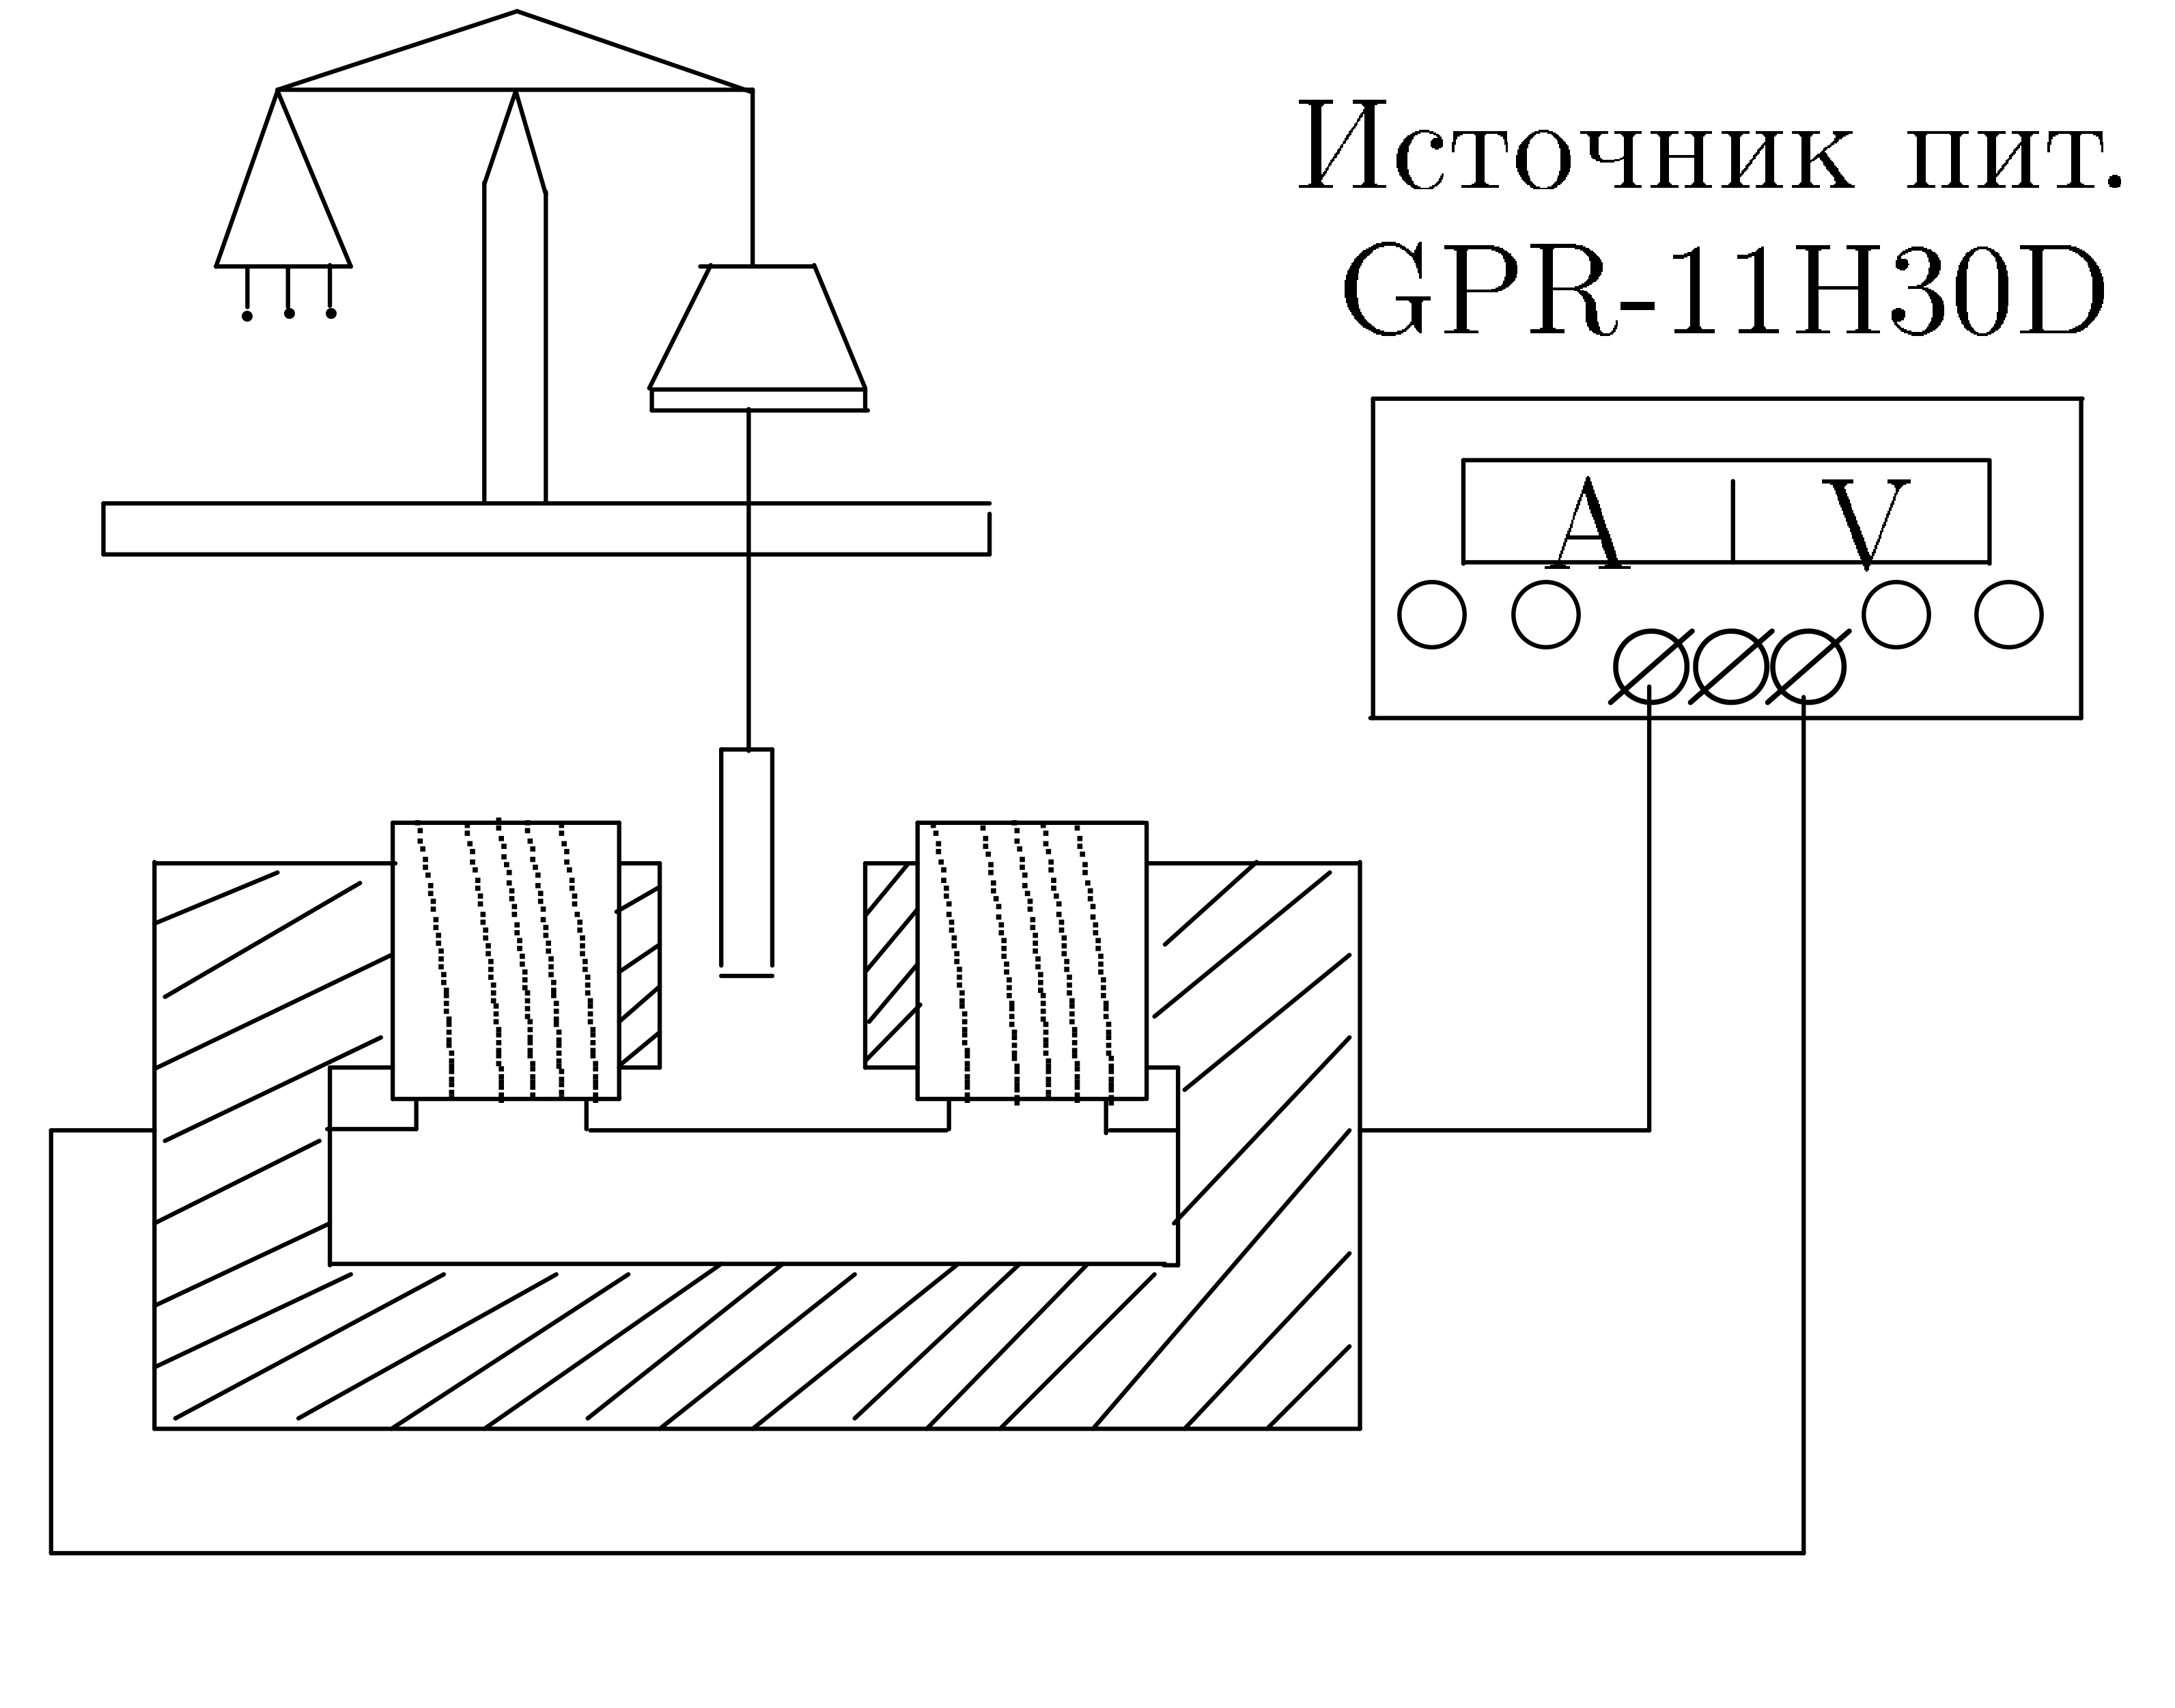
\includegraphics[width = 0.22\textwidth]{Pct1}
\captionsetup{justification = centering}
\caption{Схема установки \label{Fig1}}
\end{wrapfigure}

\paragraph{Экспериментальная установка.} Схема установки изображена на рисунке 1. Магнитное поле индукцией $B$ создается с помощью электромагнита, питаемого постоянным током силой $I$. Т.к. зависимость $B(I)$ изначально неизвестна, было необходимо построить калибровочную кривую $B(I)$ и проводить дальнейшие измерения при тех же самых токах. Ток измеряется амперметром, индукция поля~--- милливеберметром. Измеряется поток $\Phi_1$ внутри электромагнита и $\Phi_0$ вдали от него, после этого получаем индукцию поля по формуле
\begin{equation}
B = \frac{\Phi_1-\Phi_0}{NS}\label{bexp},
\end{equation}
где $N$ - число витков катушки милливеберметра, $S$ - площадь поперечного сечения. В этом эксперименте
\begin{equation}
NS = 72~\text{см}^2.
\end{equation}
\begin{table}[h!]\centering
\begin{tabular}{|*{9}{c|}}
\hline
$I, \text{А}$&0,40&0,80&1,20&1,60&2,00&2,40&2,00&3,16\\
\hline
$\Phi_1, \text{мВб}$&2,7&3,3&4,1&4,8&5,5&6,1&6,7&7,0\\
\hline
$\Phi_0, \text{мВб}$&1,6&1,4&1,2&1,0&0,9&0,6&0,5&0,2\\
\hline
$B, \text{Тл}$&0,14&0,24&0,37&0,49&0,59&0,71&0,80&0,87\\
\hline
\end{tabular}
\caption{Измерения $I(B)$}
\end{table}
\paragraph{Обработка результатов.} Результаты измерений и пересчитанные значения занесены в таблицу 1. Погрешности $\Phi_1$ и $\Phi_0$ приняты
\begin{equation}
\Delta \Phi = 0,05~\text{мВб}.
\end{equation}
Отсюда, в силу (\ref{bexp}) находится погрешность $B$~--- $\Delta B$:
\begin{equation}
\Delta B = \sqrt{2}\frac{\Delta \Phi}{NS} \approx 0,01~\text{Тл}.
\end{equation}

\begin{wrapfigure}{r}{0.53\textwidth}
\centering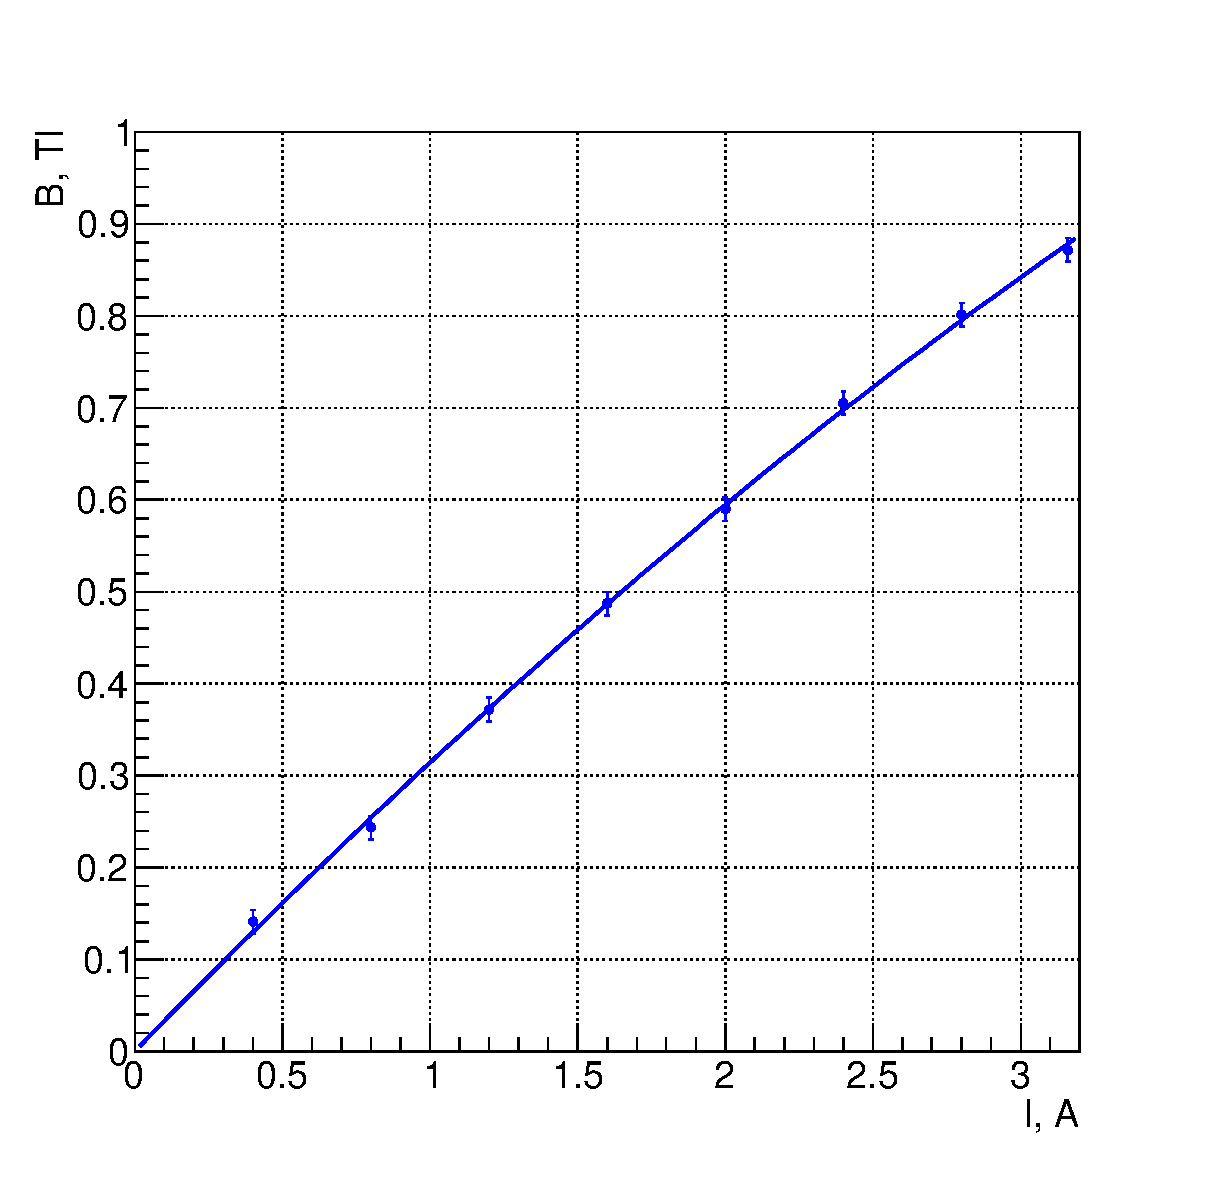
\includegraphics[width = 0.53\textwidth]{Plt1}
\captionsetup{justification = centering}
\caption{График зависимости $B(I)$\label{Fig2}}
\end{wrapfigure}
График $B(I)$ представлен на рис. 2. Вообще говоря, в силу закона Био-Савара-Лапласа, зависимость должна быть прямой пропорциональностью. Но, как мы видим, при токах наблюдаются отклонение, поэтому было использовано следующее фитирование:
\begin{equation}
I = \alpha B+\beta B^2
\end{equation}
Как мы видим, эта зависимость хорошо ложится на экспериментальные данные, для нее $\chi^2 \approx 2$ (здесь $\chi$~--- \textbf{не} магнитная восприимчивость, а статистический коэффициент).
\section{Измерение магнитных восприимчивостей}
\paragraph{Экспериментальная установка.} Здесь используется та же установка, что и в предыдущей. На аналитических весах измеряется разность масс, и, таким образом, определяется вес.
\begin{equation}
|P| = |m - m_0|g,
\end{equation}
где $m$~--- показания весов, $m_0$~--- показания при отсутствии магнитного поля. Измерения проводятся при тех же токах, что были в части 2.
\begin{table}[h!]\centering
\begin{tabular}{|*{9}{c|}}
\hline
$m_{\text{ал}}, \text{г}$&0,5&3,7&7,5&16,4&24,5&33,7&43,4&50,8\\
\hline
$|P|_{\text{ал}}, \text{мН}$&0,025&0,056&0,093&0,181&0,260&0,350&0,445&0,518\\
\hline
$m_{\text{м}}, \text{мг}$&4,3&3,9&1,5&-2,3&-6,5&-10,9&-15,2&-19,7\\
\hline
$|P|_{\text{м}}, \text{мН}$&0,022&0,026&0,049&0,086&0,128&0,171&0,213&0,257\\
\hline
$m_{\text{гр}}, \text{мг}$&-5,9&-13,9&-29,2&-49&-69,8&-97,7&-119,6&-147,4\\
\hline
$|P|_{\text{гр}}, \text{мН}$&0,034&0,113&0,263&0,458&0,662&0,936&1,151&1,424\\
\hline
$B^2, \text{Тл}^2$&0,020&0,059&0,138&0,237&0,348&0,497&0,642&0,760\\
\hline
$\Delta B^2, \text{Тл}^2$&0,004&0,006&0,010&0,012&0,015&0,018&0,021&0,022\\
\hline
\end{tabular}
\caption{Измерения $|P|(B)$}
\end{table}
\paragraph{Обработка результатов.} Данные эксперимента с пересчитанными значениями занесены в таблицу 2. Значком <<ал>> обозначаются соответствующие данные для алюминиевого стержня, <<м>>~--- медного, <<гр>>~--- графитового. Как мы видим, алюминий~--- парамагнегник, медь и графи~--- диамагнетики. Параметры стержней занесены в таблицу 3 ($d$ - диаметр образца).
\begin{table}[ht]\centering
\begin{tabular}{|c|c|c|c|}
\hline
~&алюминий&медь&графит\\
\hline
$m_0, \text{мг}$&-2,0&-6,5&-2,4\\
\hline
$d, \text{мм}$&10,00&10,00&6,70\\
\hline
\end{tabular}
\caption{Параметры стержней}
\end{table}
Погрешность $m$ и $m_0$ считалась равной
\begin{equation}
\Delta m = 0,1~\text{мг}.
\end{equation}
Таким образом, в силу (7), погрешность $|P|$~--- $\Delta |P|$, можно найти по формуле
\begin{equation}
\Delta |P| = \sqrt{2}\Delta m g \approx 0,002~\text{мН}.
\end{equation}
Погрешность $B^2$ (обозначена $\Delta B^2$) вычислялась по формуле
\begin{equation}
\Delta B^2 = 2\Delta B B.
\end{equation}
\begin{wrapfigure}{r}{0.53\textwidth}
\centering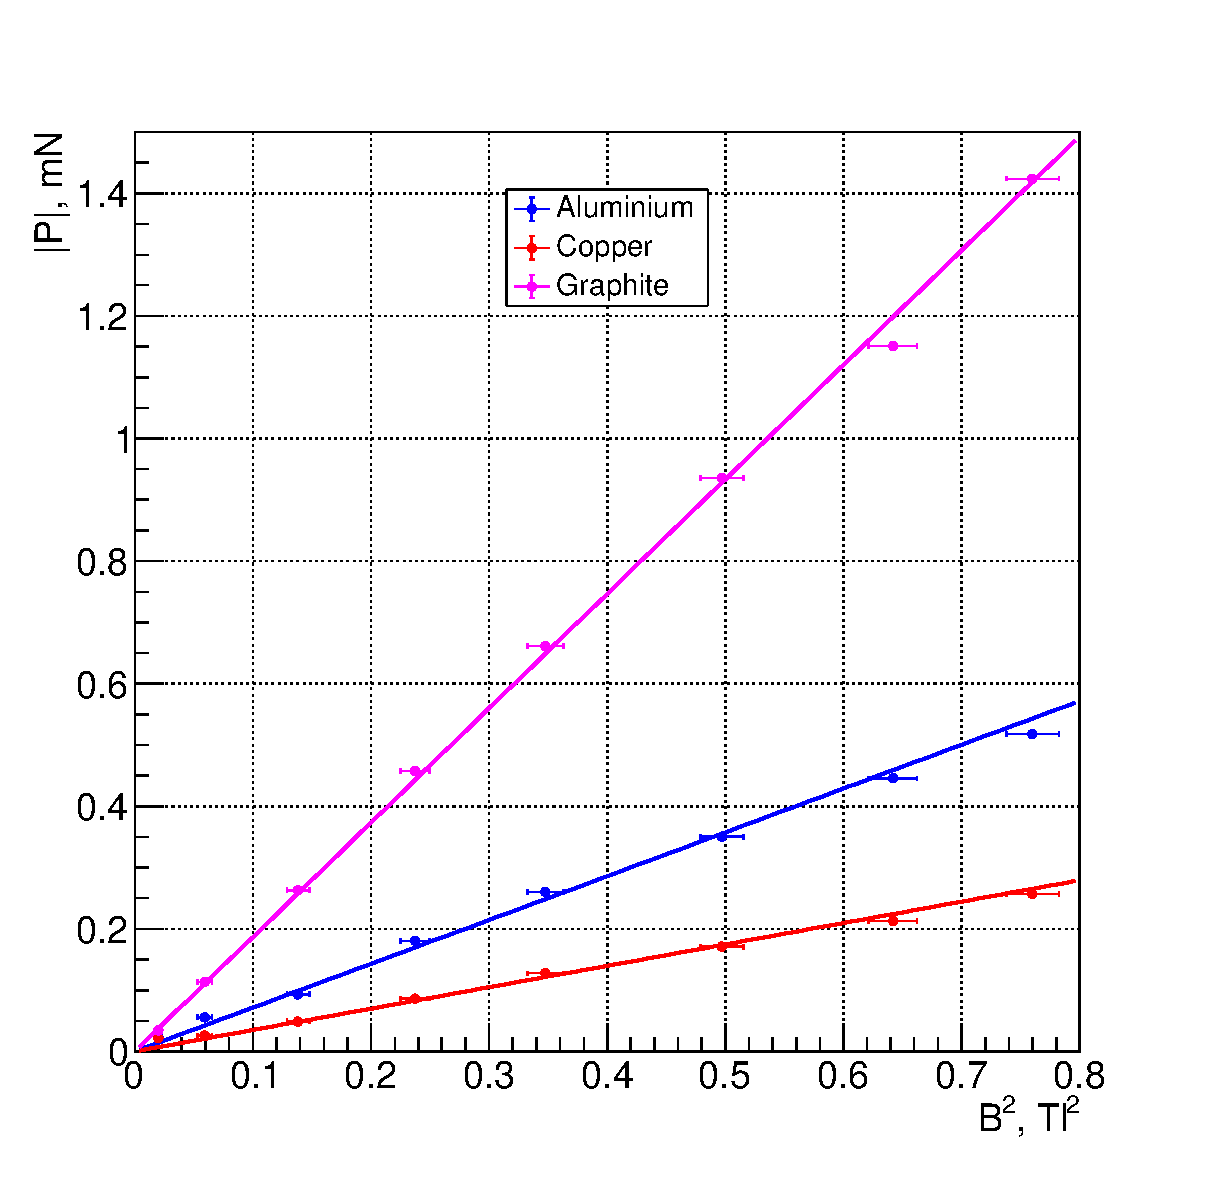
\includegraphics[width = 0.53\textwidth]{Plt2}
\captionsetup{justification = centering}
\caption{График зависимости $|P|(B^2)$\label{Fig3}}
\vspace{10pt}
\end{wrapfigure}

На рис. 3 приведен график зависимости $|P|(B)$, в легенде указана принадлежность данных тому или иному образцу. Данные были профитированы зависимостью вида
\begin{equation}
|P| = \alpha B^2.
\end{equation}
Как мы видим, данные хорошо ложатся на эти зависимости, хотя для меди и алюминия статистические коэффициенты $\chi^2 \sim20$. По формулам (1) и (3) магнитная восприимчивость определяется по формуле
\begin{equation}
|\chi| = \frac{2\alpha\mu_0\mu}{s} \approx \frac{8\alpha\mu_0}{\pi d^2},
\end{equation}
здесь мы приняли, что $\mu \approx 1$. Погрешность $\chi$, обозначаемая $\Delta \chi$, измеряется по формуле
\begin{equation}
\Delta \chi = \frac{\Delta\alpha}{\alpha}\chi,
\end{equation}
где $\Delta\alpha$~--- погрешность $\alpha$. Полученные данные занесены в таблицу 4.
\begin{table}[ht]\centering
\begin{tabular}{|c|c|c|c|}
\hline
~&алюминий&медь&графит\\
\hline
$\alpha, \text{мН}/\text{Тл}^2$&0,71&0,35&1,87\\
\hline
$\Delta \alpha, \text{Н}/\text{Тл}^2$&0,01&0,01&0,03\\
\hline
$\chi\cdot 10^{-3}, \text{мм}$&0,0227&-0,011&-0,133\\
\hline
$\Delta\chi\cdot 10^{-3}, \text{мм}$&0,0003&0,0003&0,0021\\
\hline
\end{tabular}
\caption{Магнитные проницаемости стержней}
\end{table}

Табличные значения:
\begin{equation}
\chi_\text{ал} = 2,22 \cdot 10^{-5}
\chi_\text{м} = -1,03\cdot 10^{-5},
\end{equation}
что хорошо совпадает с полученными значениями.
\section{Заключение}
Все цели работы достигнуты, магнитные восприимчивости образцов были определены с достаточно высокой точностью (совпали с табличными).
\end{document}